\item Un tanque, de radio $R$ y altura $H$, se encuentra ubicado en posición vertical con su interior repleto de agua. Como se observa en la figura \ref{fig:tanque_vert} consisten en dos mitades cilíndricas. Ambas mitades son sujetadas por medio de tornillos. Determinar la fuerza que realiza cada tornillo, si la separación entre ellos es L. ¿Qué tornillos son sometidos a la mayor carga?¿Cómo puede estimar cuál es la diferencia de carga en cada tornillo?. Las variables del problema son:
%% Esto son datos centrados
\begin{center}
%$\R = 2 \{m} \H = 4 \{m} $\\
%$\L = 50 \{cm} \
$R \qquad H \qquad \rho \qquad L$
\end{center}
%% Esto es una figura

\begin{figure}[h!!!!]
\centering
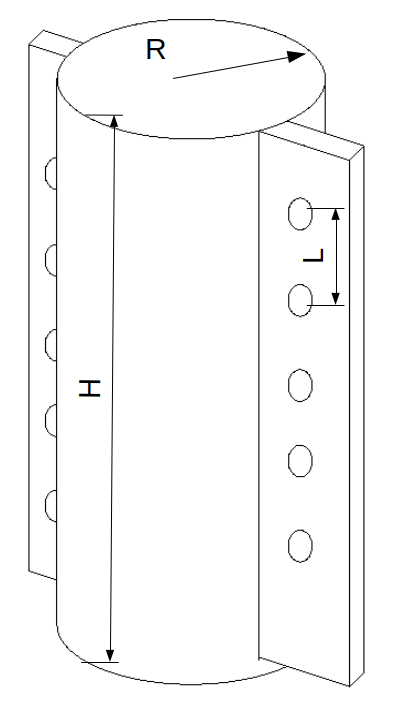
\includegraphics[width=0.3\textwidth]{cilindrico_vertical.png}
\caption{tanque cilindrico vertical}
\label{fig:tanque_vert}
\end{figure}
